% fixture: templates/lab-report
% oracle: pdflatex
% files: setup.jpg plot.png
% tier: T3
% engine: document
% covers: the lab report template: \maketitle, siunitx's \SI with a ± uncertainty, a booktabs tabular with @{} and \multirow in a [h] table, two subcaption subfigures holding a JPEG and a PNG at \linewidth under pdflatex, caption.sty's captions
% issue: #271
% source: packages/engine/corpus/lab-report.tex
\documentclass{article}
\usepackage{siunitx}
\usepackage{booktabs}
\usepackage{multirow}
\usepackage{caption}
\usepackage{subcaption}
\usepackage{graphicx}

\title{Lab 4: Pendulum Period}
\author{Group 7}

\begin{document}
\maketitle

\section{Aim}
Measure the period of a simple pendulum of length \SI{0.75}{\metre}.

\section{Data}
\begin{table}[h]
  \centering
  \begin{tabular}{@{}lrr@{}}
    \toprule
    Trial & Period (s) & Error (s) \\
    \midrule
    \multirow{2}{*}{A} & 1.74 & 0.02 \\
                       & 1.73 & 0.02 \\
    B & 1.75 & 0.01 \\
    \bottomrule
  \end{tabular}
  \caption{Measured periods.}
\end{table}

\begin{figure}[h]
  \centering
  \begin{subfigure}{0.45\textwidth}
    
\includegraphics[width=\linewidth]{setup.jpg}
    \caption{Setup}
  \end{subfigure}
  \begin{subfigure}{0.45\textwidth}
    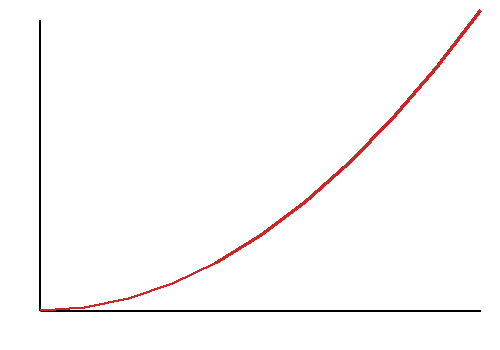
\includegraphics[width=\linewidth]{plot.png}
    \caption{Period vs length}
  \end{subfigure}
  \caption{The experiment.}
\end{figure}

\section{Conclusion}
The mean period is \SI{1.74 \pm 0.02}{\second}, close to the predicted value.
\end{document}
